\section{A new approach}
Splitting the \obs interface into a base interface that is focuses on hot sources and a subinterface that is optimized for cold asynchronous sources brings up the issue of how much to put in this subinterface. After all, the contract of the producer of the data being in charge and the consumer reacting to the received data is already in the base interface, just as the operators that gives Rx its great value of compositionality and its ability to do asynchronous computations.

One way to go is to implement backpressure in this subinterface as envisioned by Reactive Streams. This however would require an implementation like `post v.0.20' RxJava with the \code{Producer} interface added to to the architecture as well as a reimplementation of the operators that require backpressure support. Note that this implies that within the operator sequence the stream would be interactive rather than reactive. Also note that we already discussed some problems with this implementation in \Cref{subsec:handling-overproduction-with-reactive-streams,subsec:handling-overproduction-with-rxjava}.

As pointed out by the RxJava wiki \cite{RxJava-Wiki-Backpressure}, backpressure does not make the problem of an overproducing source go away. It only moves the problem up the chain of operators to a point where it can be handled better. This means that a \code{request(n)} call from the \code{zip} operator in \Cref{sec:fastproc-slowcons} goes up the chain to the point where it can fulfill that request. This is either an operator like \code{onBackpressureBuffer} or \code{onBackpressureDrop} or the source that is wrapped in an \code{Observable.create} or one of its higher abstractions.

Another way to go with the implementation of the subinterface is to decouple the flow control from the operators and move it to the origin of the stream. This way we can keep the API clean, we do not have to take this flow control into account while implementing new operators, we do not have to reimplement the operators inherited from the base interface and (most importantly) we can keep the operator sequences reactive.

For this approach we need to observe that the \obs is nothing more than just a source wrapped in \code{Observable.create}, from which this source instantly gains all the operators, the possibility to go asynchronous and to potentially be composed with other sources using operators such as \code{flatMap}, \code{combineLatest}, \code{withLatestFrom} and \code{zip}.

Instead of wrapping a cold source in the \code{Observable.create} as is currently done in RxJava, we propose to wrap it in a universal interactive interface (such that communication with the source is not coupled with its own specific interface) and let a function equivalent to to \code{Observable.create} pull the data out of the source via this interface on behalf of the one who subscribes. The data is then put into a bounded buffer, from which it is pulled again by a downstream \obs that operates on a different thread. Once an element is pulled from the buffer, it will block the downstream \obs's callstack from pulling another element until the current element is fully processed or taken over by a third thread. In the mean time the buffer can request new elements from the source and by doing so keeps the downstream \obs as busy as it possibly can without letting it wait for a new element to be produced by the source.

\begin{figure}[H]
	\begin{center}
		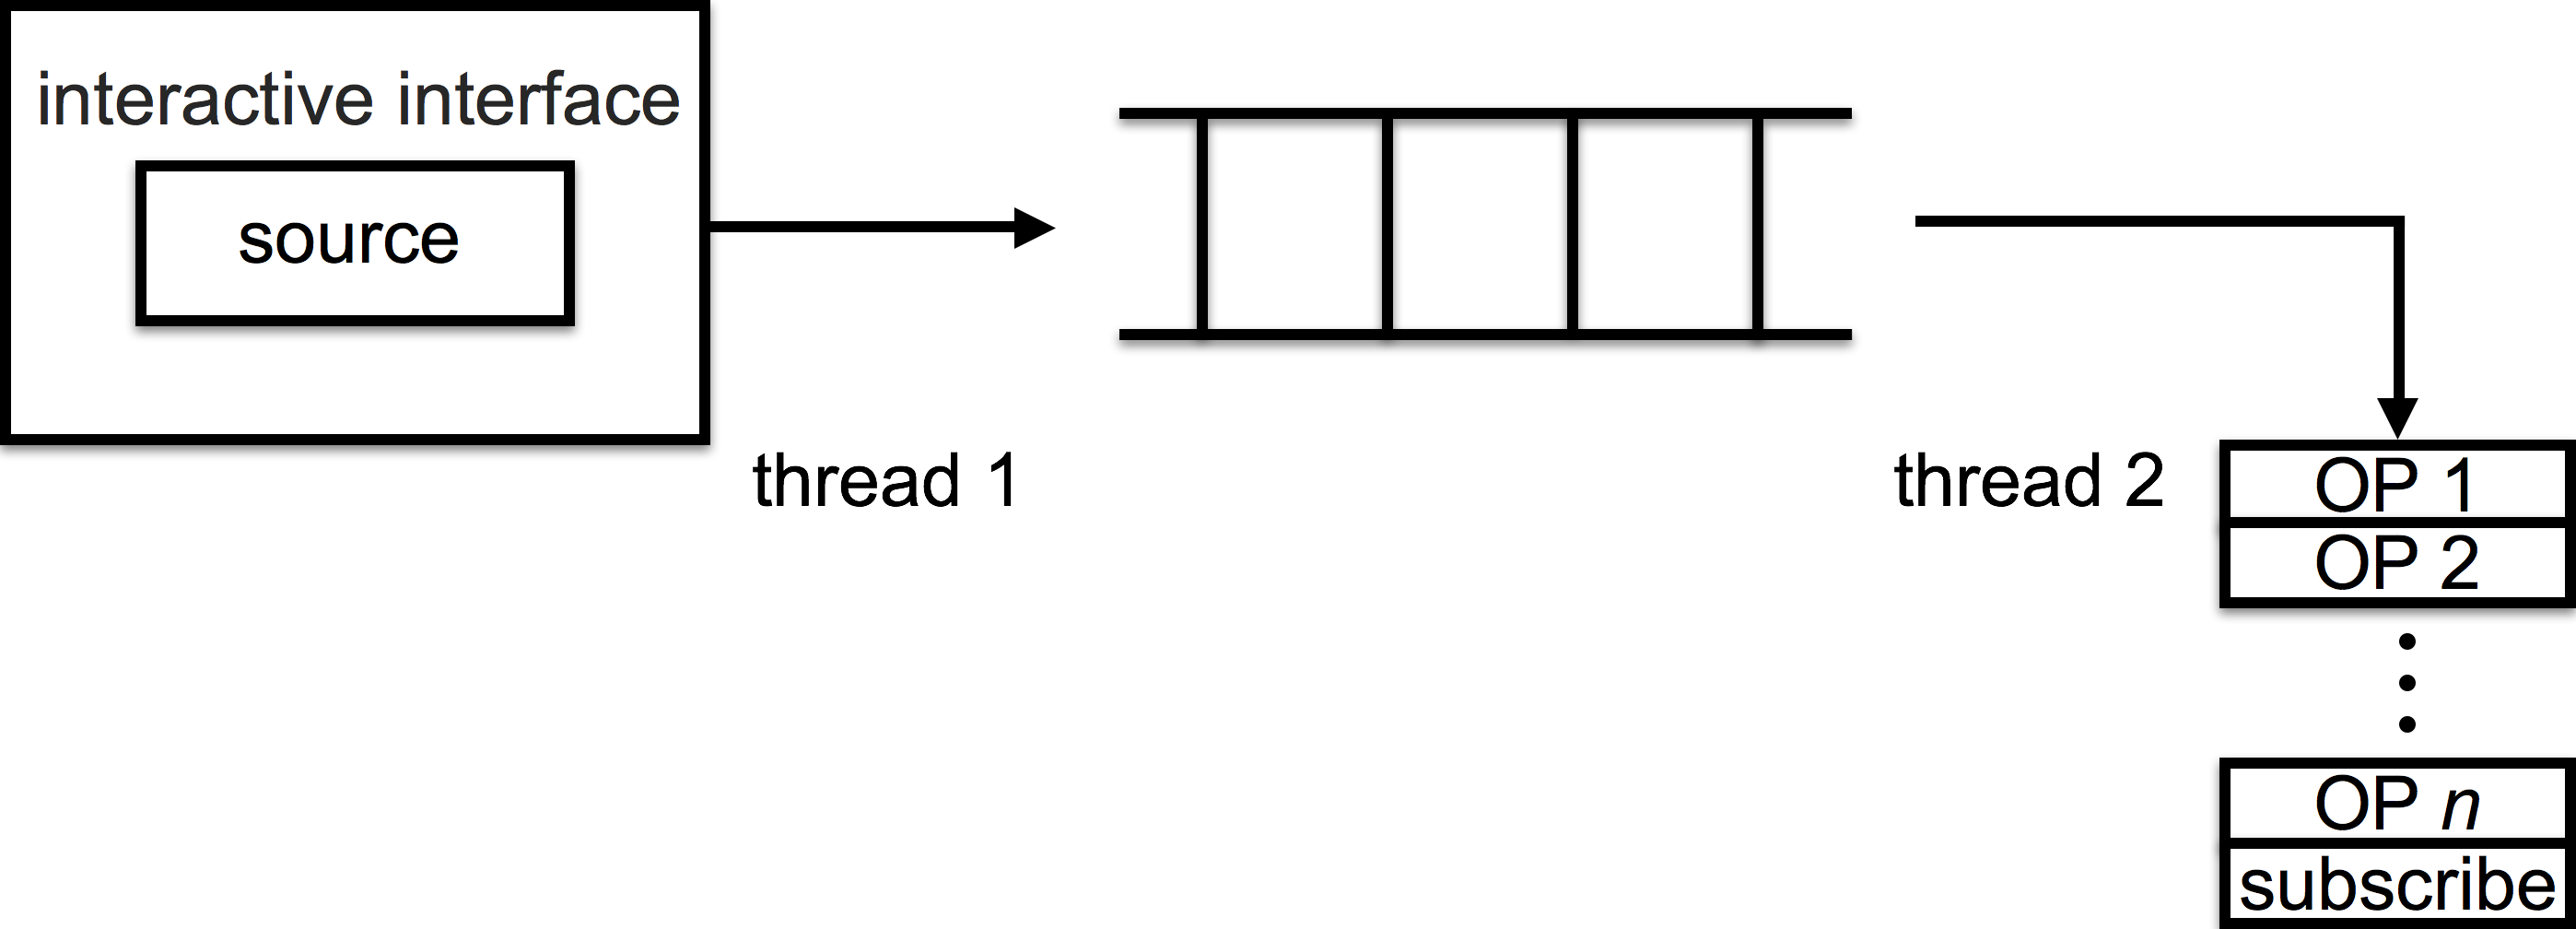
\includegraphics[width=0.63\textwidth]{figures/Approach.png}
	\end{center}
	\caption{Schematic representation of our approach}
	\label{fig:new-approach}
\end{figure}

With this approach we have reduced the problem of overproduction to a problem of controlling the size of a buffer to be as small as possible, without the buffer being exhausted by a fast consuming downstream. A buffer size that is too small can lead to a needless delay in consuming the data, whereas a too large buffer size is not desirable as well, given that we want to spend as little resources as possible. The complicating factor here is that it is unknown at all times how long it will take for the source to produce a next element.

In order to overcome this unknown factor, control the size of the buffer and only request new elements from the source when needed, we will use a well-known technique from mechanical and electrical engineering called \textit{feedback control}. Since this is a technique that is unfortunately not as well-known in computer science and software engineering as it is in other parts of science and engineering, we will introduce this technique in the upcoming chapters, develop an API to work with this technique in general and present the rest of our solution to the overproduction problem after that.

Obviously RxJava in its current stage cannot be used to implement this solution, as it already has a backpressure implementation. Therefore we will use the RxMobile \cite{RxMobile} reference implementation which was recently written in Scala by Erik Meijer as a basic API for reactive programming and build our approach on top of that without the need of rewriting any existing code.
